
%(BEGIN_QUESTION)
% Copyright 2006, Tony R. Kuphaldt, released under the Creative Commons Attribution License (v 1.0)
% This means you may do almost anything with this work of mine, so long as you give me proper credit

Graph the response of an hypothetical {\it derivative-only} controller for the following input conditions.  Assume a control action that is {\it direct-acting}, and a derivative constant ($\tau_d$) of 2 minutes:

$$\includegraphics[width=15.5cm]{i01545x01.eps}$$

The time scale on the chart is minutes:seconds, and the algorithm for this controller is as follows:

$$m = \tau_d {de \over dt} + b$$

\noindent
Where,

$m$ = Controller output (manipulated variable)

$e$ = Error signal (PV$-$SP)

$\tau_d$ = Derivative time constant

$b$ = Bias

\vskip 10pt

\underbar{file i01545}
%(END_QUESTION)





%(BEGIN_ANSWER)

$$\includegraphics[width=15.5cm]{i01545x02.eps}$$

%(END_ANSWER)





%(BEGIN_NOTES)



%INDEX% Control, derivative: graphing controller response

%(END_NOTES)


